\documentclass{puzzlehunt}

\usepackage[final]{pdfpages}
\usepackage{amsmath,amssymb}
\usepackage{pgf,tikz}
\usetikzlibrary{arrows}

\usepackage{array}

\usepackage{environ}

\usepackage{chessfss}

\usepackage{multicol}
\usepackage{multirow}


% Contest name macros
\newcommand{\phEventName}{Mathematical Puzzle Programs}
\newcommand{\phEventAbbr}{Mathematical Puzzle Programs}


\title{\phEventName}
\author{Mathematical Puzzle Programs}
\date{\today}

% \phMarkDraft

\phSetSquareLogo{assets/mapp-square.pdf}
\phSetBannerLogo{assets/mapp-banner.pdf}

\begin{document}

\phChapterWorksheet{Getting on Top of Things}{Example Puzzle}

A friend passes you a note with the following strange image.

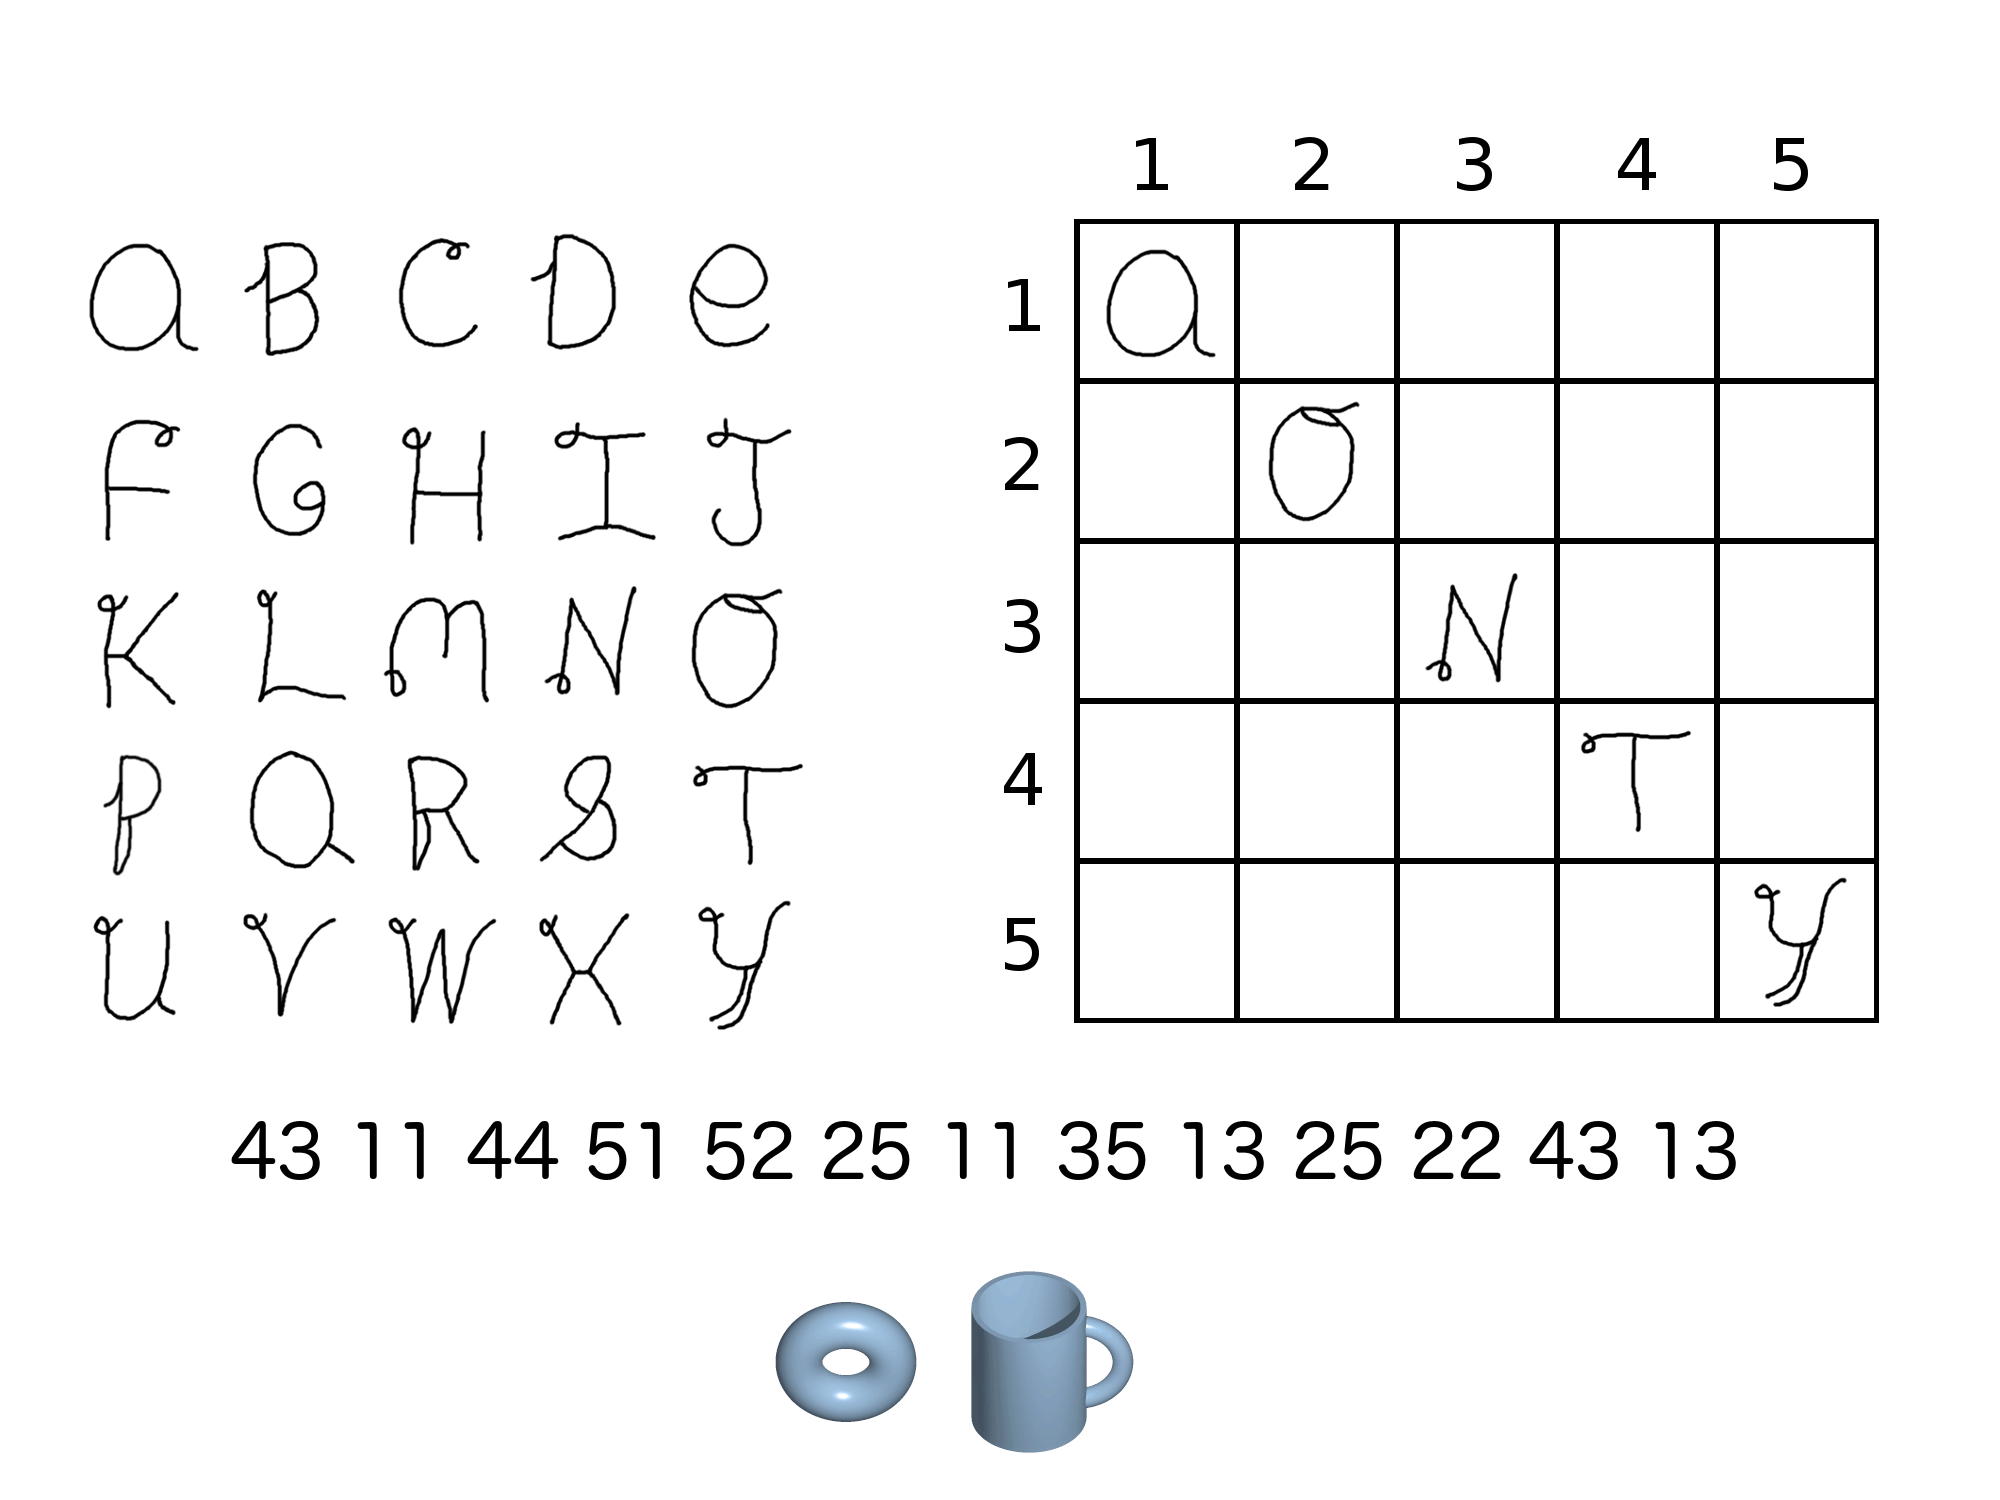
\includegraphics[width=0.9\linewidth]{assets/topology-puzzle.png}

She's recently been interested in \textbf{topology}, the study of structures
that can be morphed from one to another without cutting or tearing, such as
the donut and coffee cup shown in the image.
\textit{Can you decode the number pairs by finding five groups of
topologically-equivalent letters? Try writing each group in alphabetical
order on the corresponding rows of the grid...}

\phChapter{About MaPP}

The mission of Mathematical Puzzle Programs (MaPP) is to organize quality events
which get students having fun by learning and using mathematics.

\begin{itemize}
\item \textbf{Math}\newline
Our mathematical content is pulled from various areas unrepresented in the
usual secondary curriculum,
such as design theory, game theory, or topology.

\item \textbf{Puzzles}\newline
We shredded the multiple choice tests, and instead designed several
mathematical puzzles which will
give your students a taste of real mathematical problem solving, and prepare
them for the types of questions asked in many job interviews.

\item \textbf{Team-Building}\newline
MaPP features a team-based competitions, emphasizing collaboration and
communication over individual work, as teamwork is crucial for success in both
industry and academia.

\item \textbf{FUN!}\newline
Many of the challenges can't be solved sitting down - players will find
themselves running around their
host campus to track down clues and uncover new puzzles to solve.
\end{itemize}

\phSection{Programs}

\begin{itemize}
\item \textbf{High School Challenge}\newline
A game for 9th-12th grade students which showcases the fun of mathematics
as well as featuring the host campus with a customizable opening puzzle.

\item \textbf{Middle School Challenge}\newline
A game for 6th-8th grade students perfect for inspring younger audiences to
engage in mathematics.
\end{itemize}

\vspace{0.8em}

\begin{multicols}{2}
  \phSection{How to Get Involved}

  \begin{itemize}
  \item Become a MaPP partner campus!
  \item Contribute a puzzle!
  \item Spread the word!
  \item Visit or volunteer at a competition near you!
  \item Download our free puzzle materials!
  \end{itemize}

  \columnbreak

  \phSection{Contact}

  \begin{itemize}
  \item Web: MaPPmath.org
  \item Twitter: @MaPPmath
  \item Email: director@mappmath.org
  \item Email: communications@mappmath.org
  \end{itemize}
\end{multicols}

\end{document}

%%% Local Variables:
%%% mode: latex
%%% TeX-master: t
%%% End:
